\chapter{El Problema: Juego de Distribuci\'on de la Cerveza}

%The purpose of the game is to understand the distribution side dynamics of a multi-echelon supply chain used to distribute a single item, in this case, cases of beer.


%There is a one-point cost for holding excess inventory and a one-point cost for any backlog (old backlog + orders - current inventory).

%The game is used to illustrate one of the links between System Dynamics theory and the Feedback Control Theory which inspired it - that systems with positive feedback loops and high gain can lead to oscillation and overload,

La estructura se puede observar en la figura \ref{diagram_wikipedia}.\footnote{Imagen tomada de la página de Wikipedia \textit{The Beer Distribution Game}, bajo la licencia Creative Commons Attribution-Share Alike 3.0 Unported}\\


\begin{figure}[h]
\caption{Distribución de Cerveza}
\label{diagram_wikipedia}
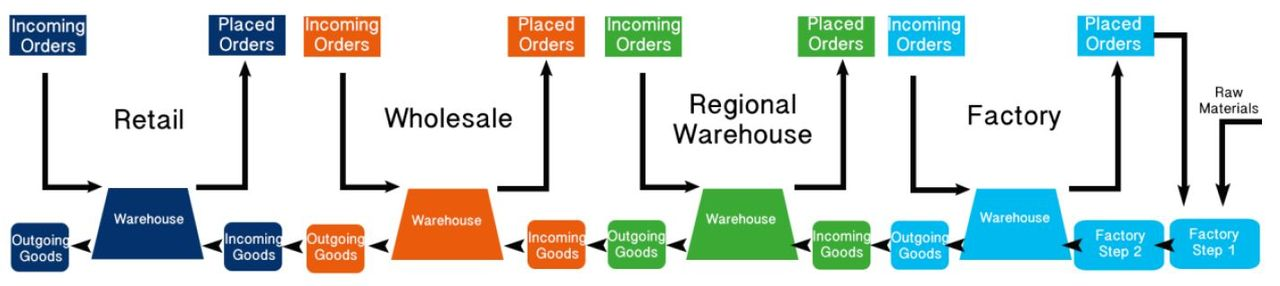
\includegraphics[width=8cm]{Diagrama_Wikipedia.JPG}
\centering
\end{figure}

Las variables que tienen efecto en este problema son:
\begin{itemize}
    \item Demanda del Consumidor
    \item Tiempo de Ajuste de Inventario
    \item Tiempo de Envío
    \item Tiempo de Producción
\end{itemize}

Para cada uno de los agentes: tiendas minorista, mayorista y de distribución, y fábrica.\\

Este problema se ha estudiado antes por \citet{Strozzi}, por medio de Algoritmos Genéticos y por \citet{Chaharsooghi} por medio de $Q-learning$. Ambas metodolog\'ias \\

El aporte de este trabajo será agregar un componente de estacionalidad en el proveedor de la fábrica: el campo.

\subsection{\textit{Efecto Látigo}}

El \textit{Efecto Látigo} se ejemplifica con el siguiente escenario:


\begin{enumerate}
    \item El comprador, que generalmente compra $6$ cervezas, ahora quiere $10$, pero la tienda minorista solamente cuenta con $7$. El minorista le venderá todo su inventario, pues es la acci\'on que maximiza su ganancia. Debe decidir si volverá a tener un inventario de $6$ o si debe pedir un número mayor de cervezas, atendiendo la aparentemente creciente demanda. Decide pedir $9$ cervezas al siguiente nivel, la tienda de mayoreo.
    \item El mayorista cuenta con $17$ cervezas. Llena el pedido del minorista, pero decide que ten\'ia guardado demasiado inventario, as\'i que se queda con $8$ cervezas en su almac\'en, sin hacer una orden al siguiente nivel, la tienda de distribución.
    \item La tienda de distribuci\'on decide comprar $1$ unidad
\end{enumerate}

En este escenario, el mayorista obtuvo informaci\'on distorsionada acerca del repentino crecimiento en la demanda del comprador, mientras que la tienda de distribución . Si este comportamiento se mantiene durante algunos periodos más, recibiría la noticia (por medio de un incremento en las órdenes regulares) con un retraso considerable.\\

El \textit{Efecto Látigo} se refiere precisamente a este fenómeno: mientras más arriba en la cadena de suministro se encuentre un agente (es decir, más lejos del contacto directo con el comprador), más distorsionada es la información que tiene acerca de la verdadera demanda del consumidor.